% The one-time pad (notebook 51, Section 1 and Figure 1): Alice adds the key to the message bit by bit, c = m XOR k;
% the ciphertext travels over a public channel that Eve reads; Bob adds the same key, c XOR k = m. The worked example
% of Section 5 is used: m = 1011, k = 0110, c = 1101. The key has to reach Alice and Bob in advance over a private
% route: the key-distribution problem (Section 7).
\documentclass[tikz,border=6pt]{standalone}
\usepackage{amsmath,amssymb}
\usetikzlibrary{arrows.meta,positioning,calc}
\begin{document}
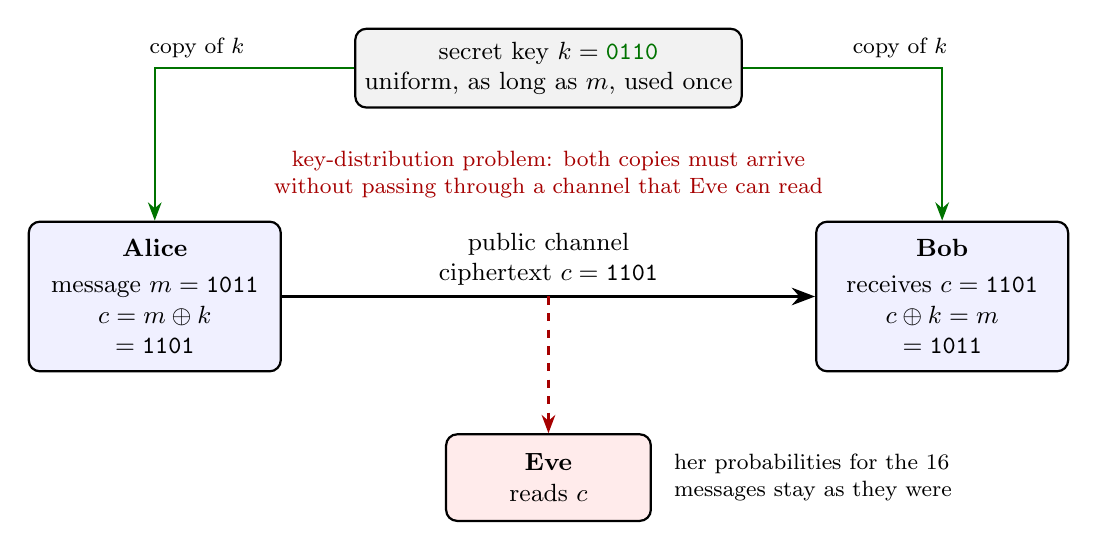
\begin{tikzpicture}[thick, >=Stealth, font=\small,
    party/.style={draw, rounded corners, fill=blue!6, minimum height=1.9cm, minimum width=3.2cm, align=center},
    adv/.style={draw, rounded corners, fill=red!8, minimum height=1.1cm, minimum width=2.6cm, align=center},
    keyb/.style={draw, rounded corners, fill=black!5, minimum height=1.0cm, minimum width=3.4cm, align=center}]
  \newcommand{\kb}[1]{\textcolor{green!45!black}{\texttt{#1}}}
  \node[party] (A) at (0,0)
       {\textbf{Alice}\\[2pt] message $m=\texttt{1011}$\\ $c=m\oplus k$\\ $=\texttt{1101}$};
  \node[party] (B) at (10,0) {\textbf{Bob}\\[2pt] receives $c=\texttt{1101}$\\ $c\oplus k=m$\\ $=\texttt{1011}$};
  \draw[->, line width=1.2pt] (A.east) --
        node[above, align=center] {public channel\\ ciphertext $c=\texttt{1101}$} (B.west);
  \node[adv] (E) at (5,-2.3) {\textbf{Eve}\\ reads $c$};
  \draw[->, dashed, red!65!black] (5,0) -- (E.north);
  \node[font=\footnotesize, align=left, right=0.15cm of E]
       {her probabilities for the $16$\\ messages stay as they were};
  % the shared key
  \node[keyb] (K) at (5,2.9) {secret key $k=\kb{0110}$\\ uniform, as long as $m$, used once};
  \draw[->, green!45!black] (K.west) -|
        node[above left, pos=0.25, font=\footnotesize, text=black] {copy of $k$} (A.north);
  \draw[->, green!45!black] (K.east) -|
        node[above right, pos=0.25, font=\footnotesize, text=black] {copy of $k$} (B.north);
  \node[font=\footnotesize, align=center, text=red!65!black] at (5,1.55)
       {key-distribution problem: both copies must arrive\\ without passing through a channel that Eve can read};
\end{tikzpicture}
\end{document}
